\section{二进制表面编码}
\label{sec:hipose_encoding}
实例级的6D物体位姿估计依赖观测图像与物体CAD模型的对应关系来估计位姿,即需要估计出观测点云或像素所对应的物体坐标系坐标。不同的物体有大有小,为了方便网络学习,我们先对物体的尺寸进行归一化,让物体坐标系的长、宽、高的尺寸均归一化为1。为了将观测图像所对应的物体坐标系坐标方便神经网络学习,将笛卡尔空间物体坐标系坐标的三个分量X、Y、Z分别用彩色图像的R、G、B的三个通道表示。\autoref{fig:坐标颜色映射}以LM-O数据集中的物体ape为例,得到物体ape在物体坐标系中X、Y、Z的最小值和最大值,并归一化到0-1空间。图中用红点标注了若干个三维包围框映射后的坐标以及物体表面映射后的坐标。
\begin{equation}
    \left\{
    \begin{aligned}
        R &= \frac{X - X_{\min}}{X_{\max} - X_{\min}} \\
        G &= \frac{Y - Y_{\min}}{Y_{\max} - Y_{\min}} \\
        B &= \frac{Z - Z_{\min}}{Z_{\max} - Z_{\min}}
    \end{aligned}
    \right.
\end{equation}
其中 下标$(\cdot)_{\min}$ 表示该分量的最小值,下标$(\cdot)_{\max}$ 表示该分量的最大值。

\begin{figure}[ht]
    \centering
    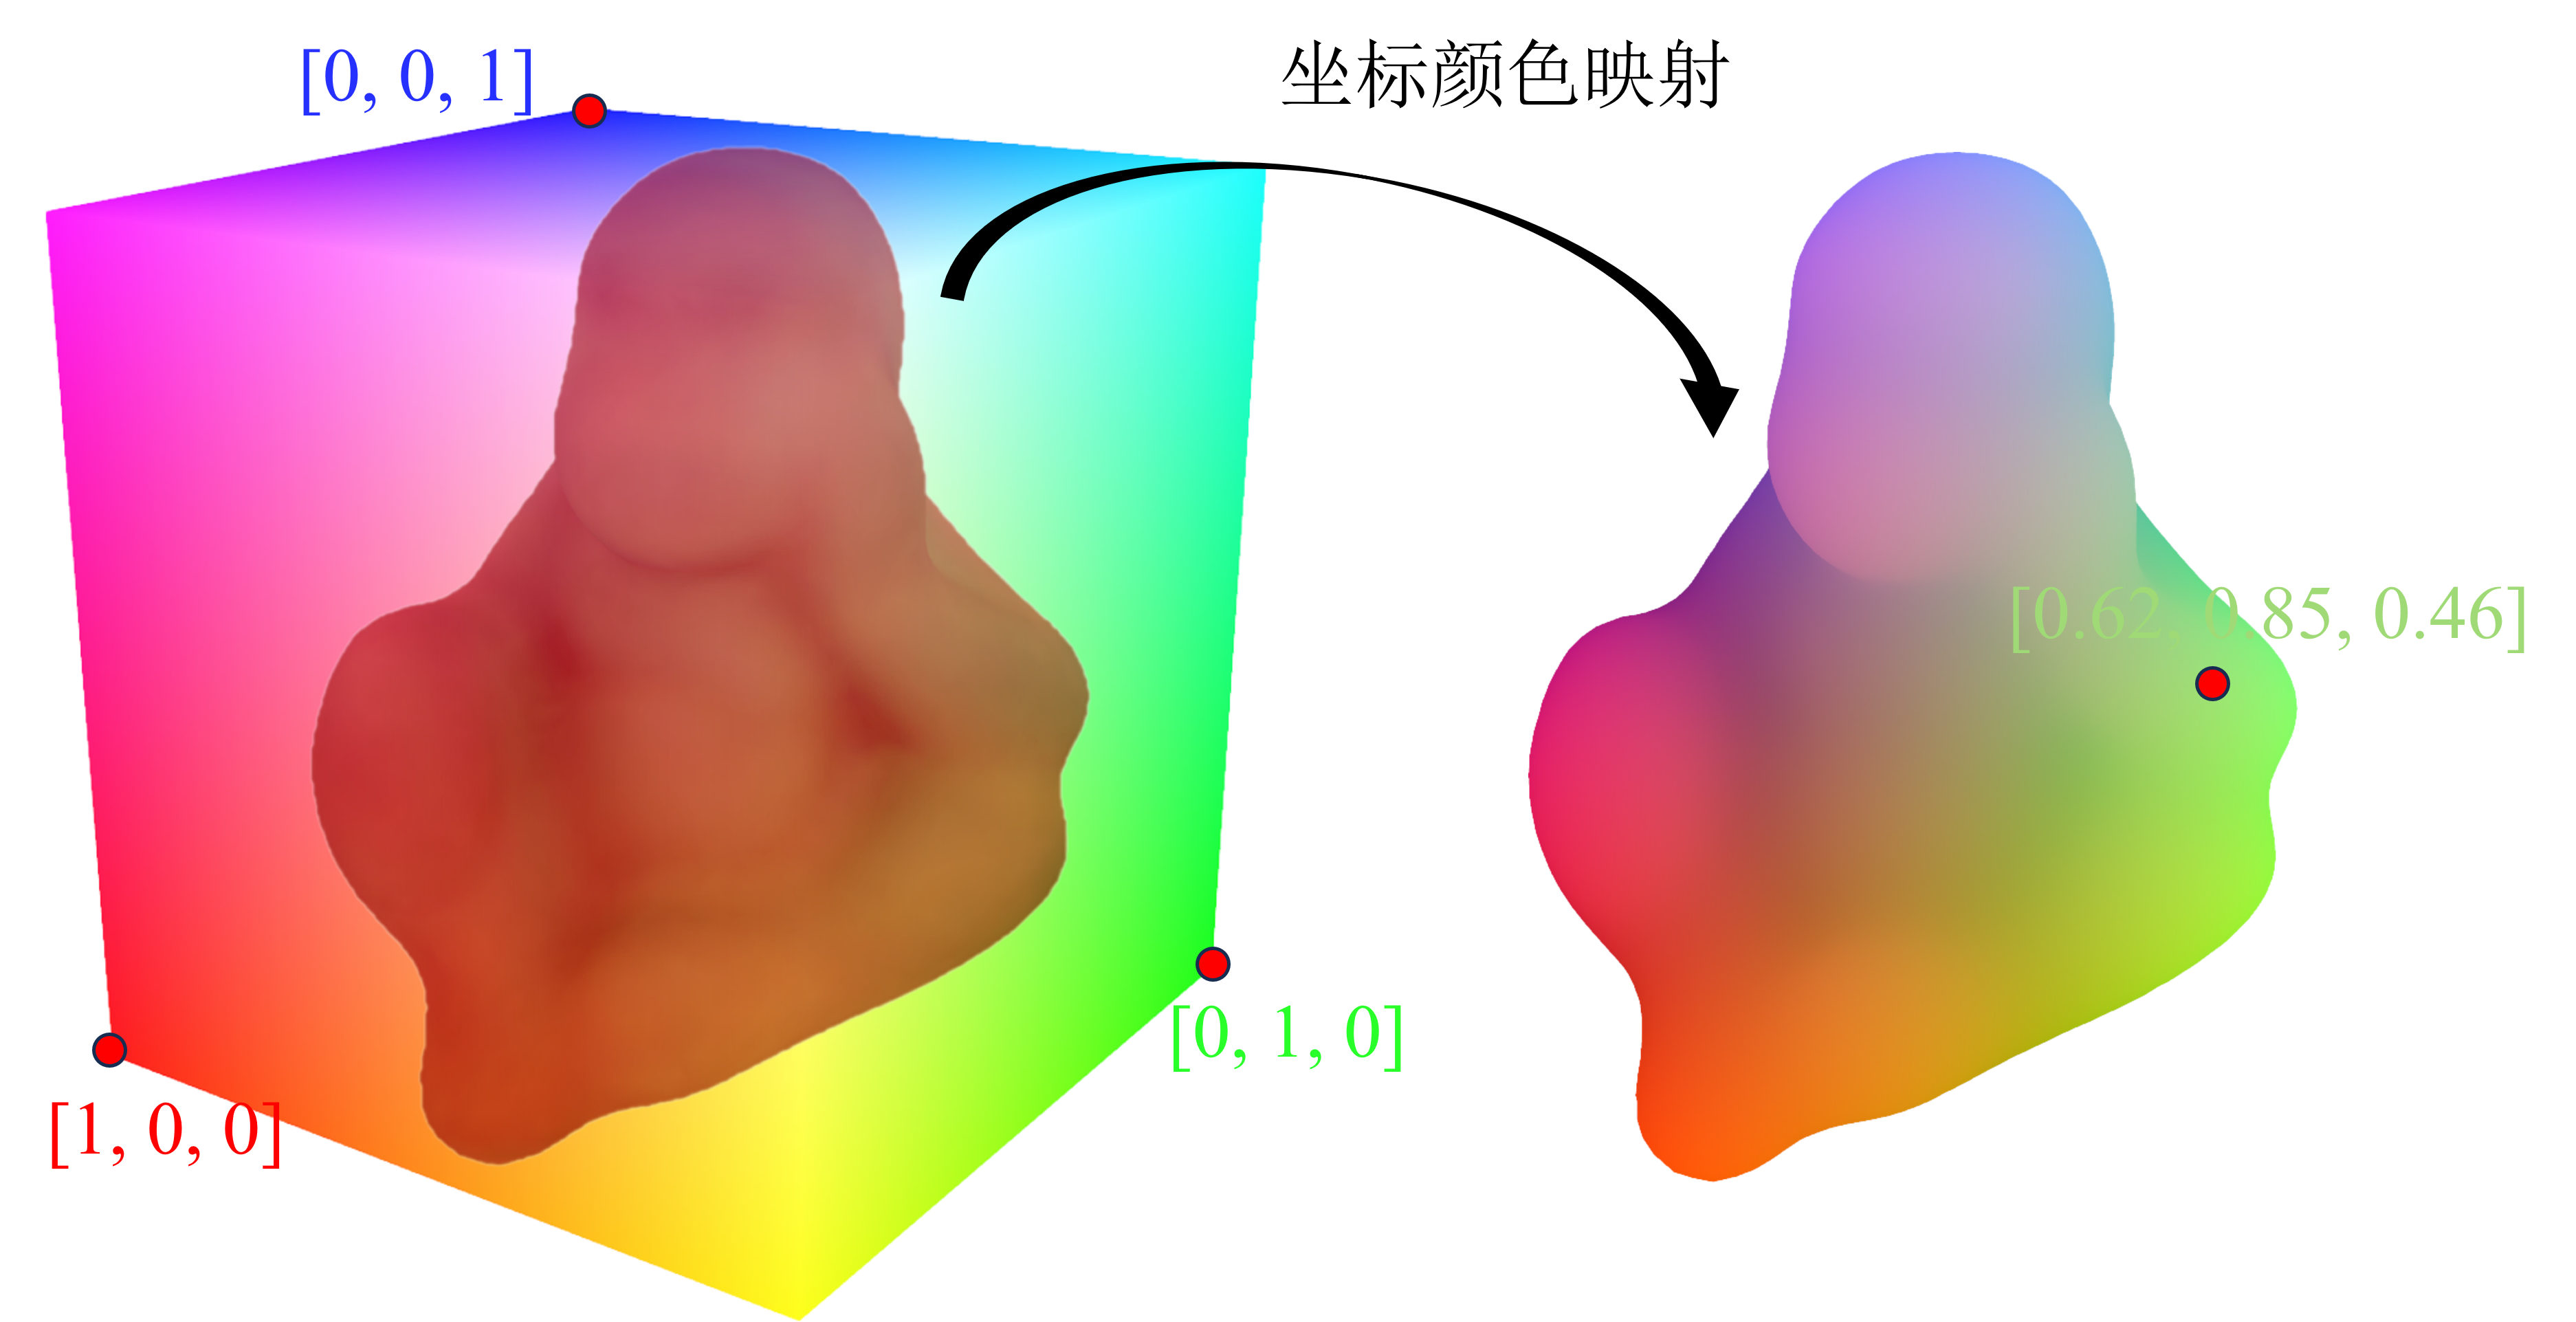
\includegraphics[width=0.75\linewidth]{hipose/坐标颜色映射.png}
    \caption{坐标颜色映射}
    \label{fig:坐标颜色映射}
\end{figure}

ZebraPose~\cite{su2022zebrapose}第一次提出使用离散的物体表面编码来替代物体表面坐标的表示方式。这种表面编码为每个顶点分配一个唯一的二进制编码,形成顶点坐标与二进制编码的一一映射。其构建流程如下。

首先,使用聚类算法迭代地将物体表面网格划分为两个部分,并为每个组分配一个比特,如\autoref{fig:聚类过程}所示。聚类步骤1将整个物体表面划分为 \ding{172} 和\ding{173} 两个部分。聚类步骤2将\ding{172}表面划分为\ding{172} 和\ding{173} 两个部分并把\ding{173}划分为\ding{174}和\ding{175}两个部分。聚类步骤3将\ding{172}划分为 \ding{172} 和\ding{173} 两个部分,以此类推。

\begin{figure}[htbp]
    \centering
    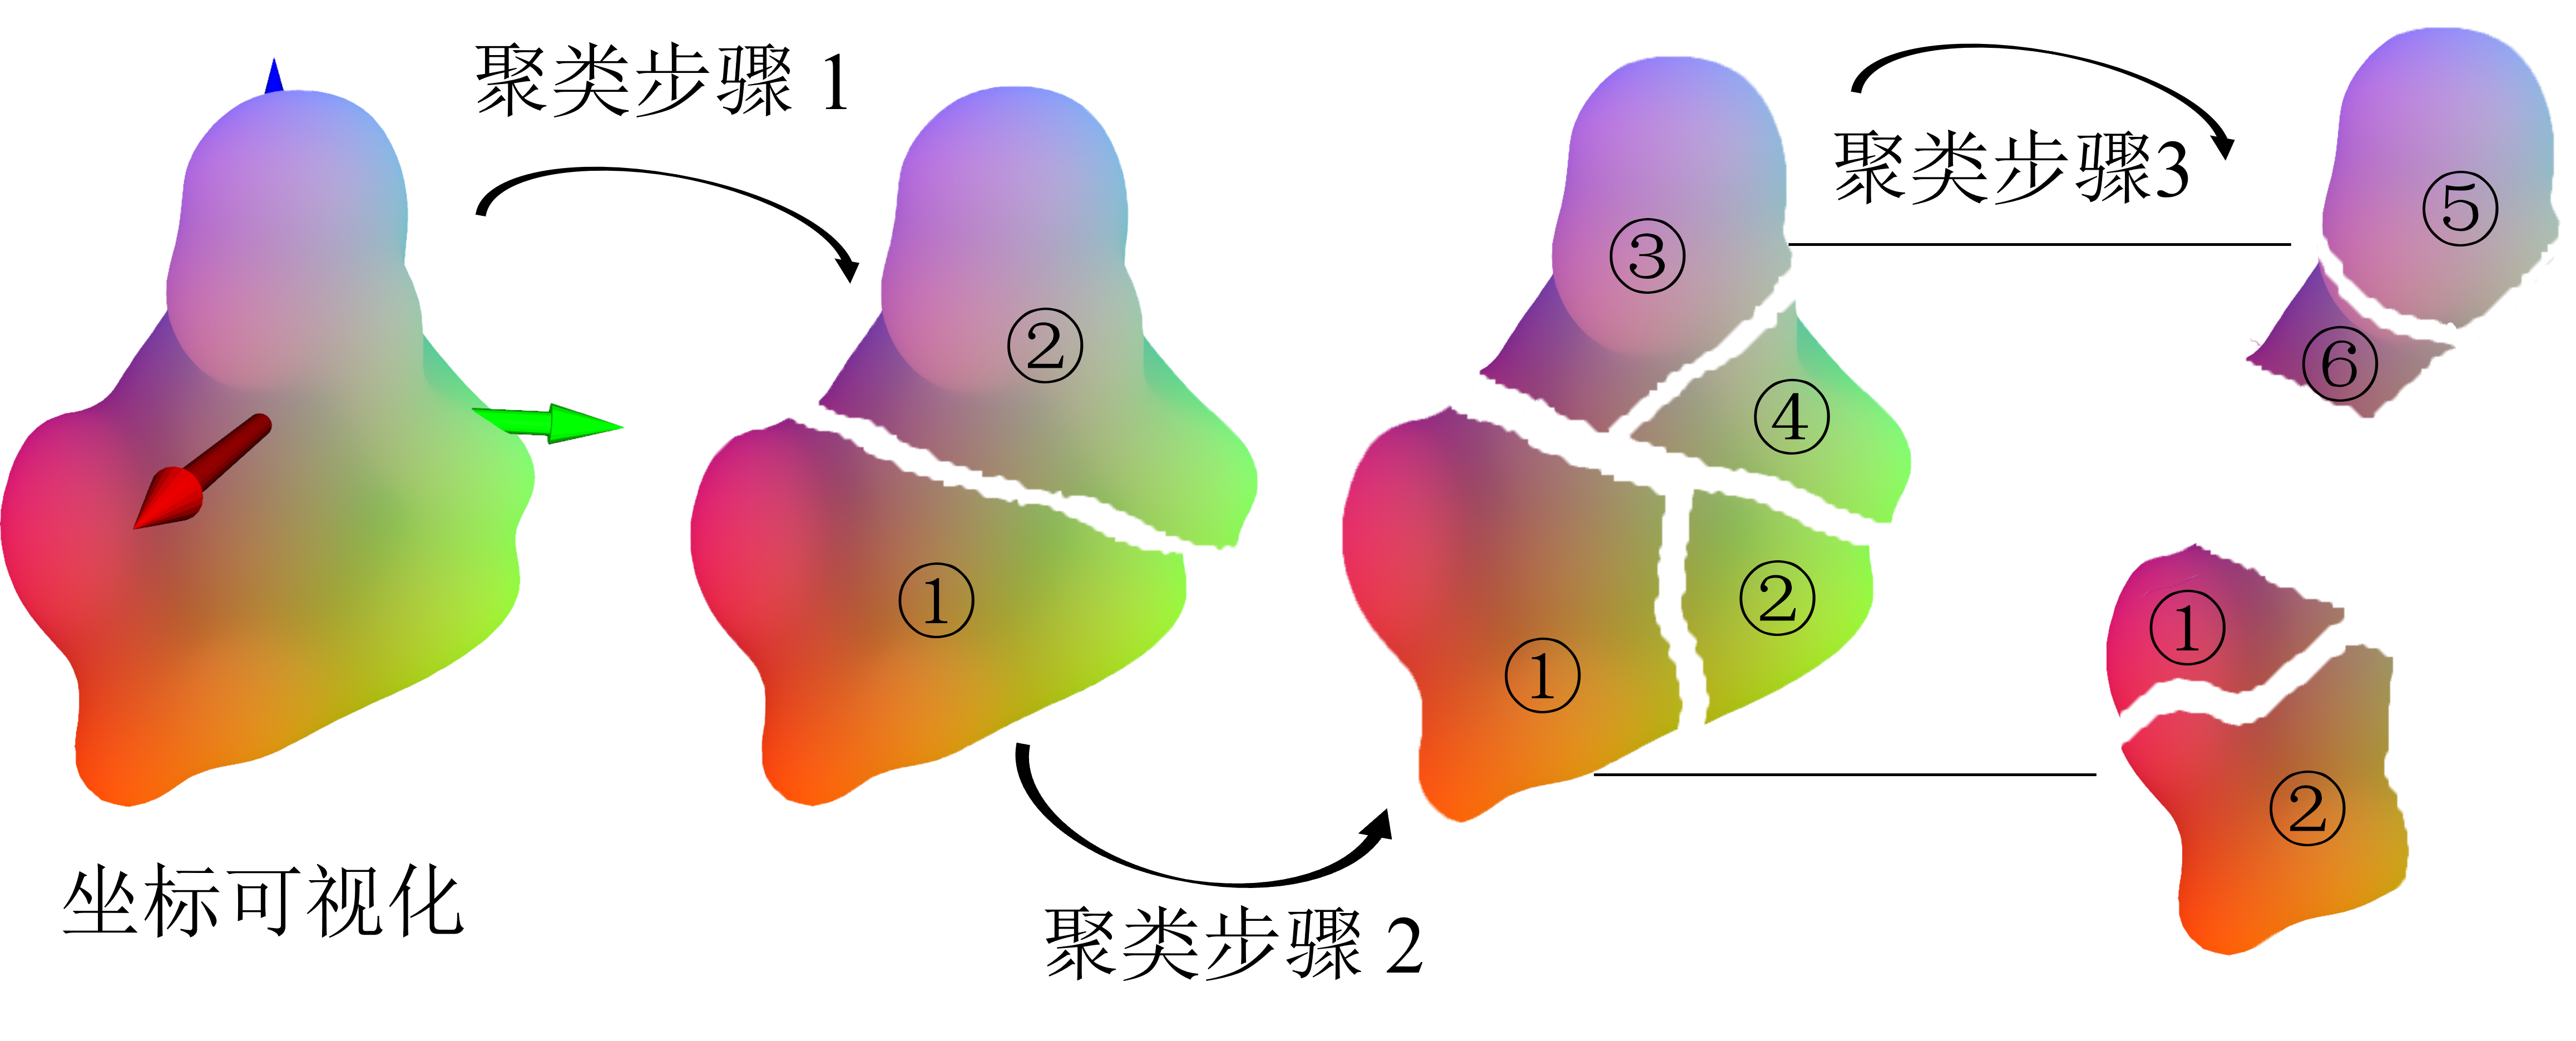
\includegraphics[width=0.75\linewidth]{hipose/聚类过程.png}
    \caption{聚类过程}
    \label{fig:聚类过程}
\end{figure}

即在第 $j, j \in \{1, \ldots, d\}$ 次表面划分迭代后,我们有 $2^{j}$ 个独立的子表面。假设一个表面包含 $L$ 个顶点,使用平衡 k-means 进行划分,结果是两个子表面分别包含 $\lfloor L/2 \rfloor$ 和 $L-\lfloor L/2 \rfloor$ 个顶点。\autoref{fig:聚类结果}展示了聚类步骤2和聚类步骤3将物体表面进行划分的结果。

\begin{figure}[htbp]
    \centering
    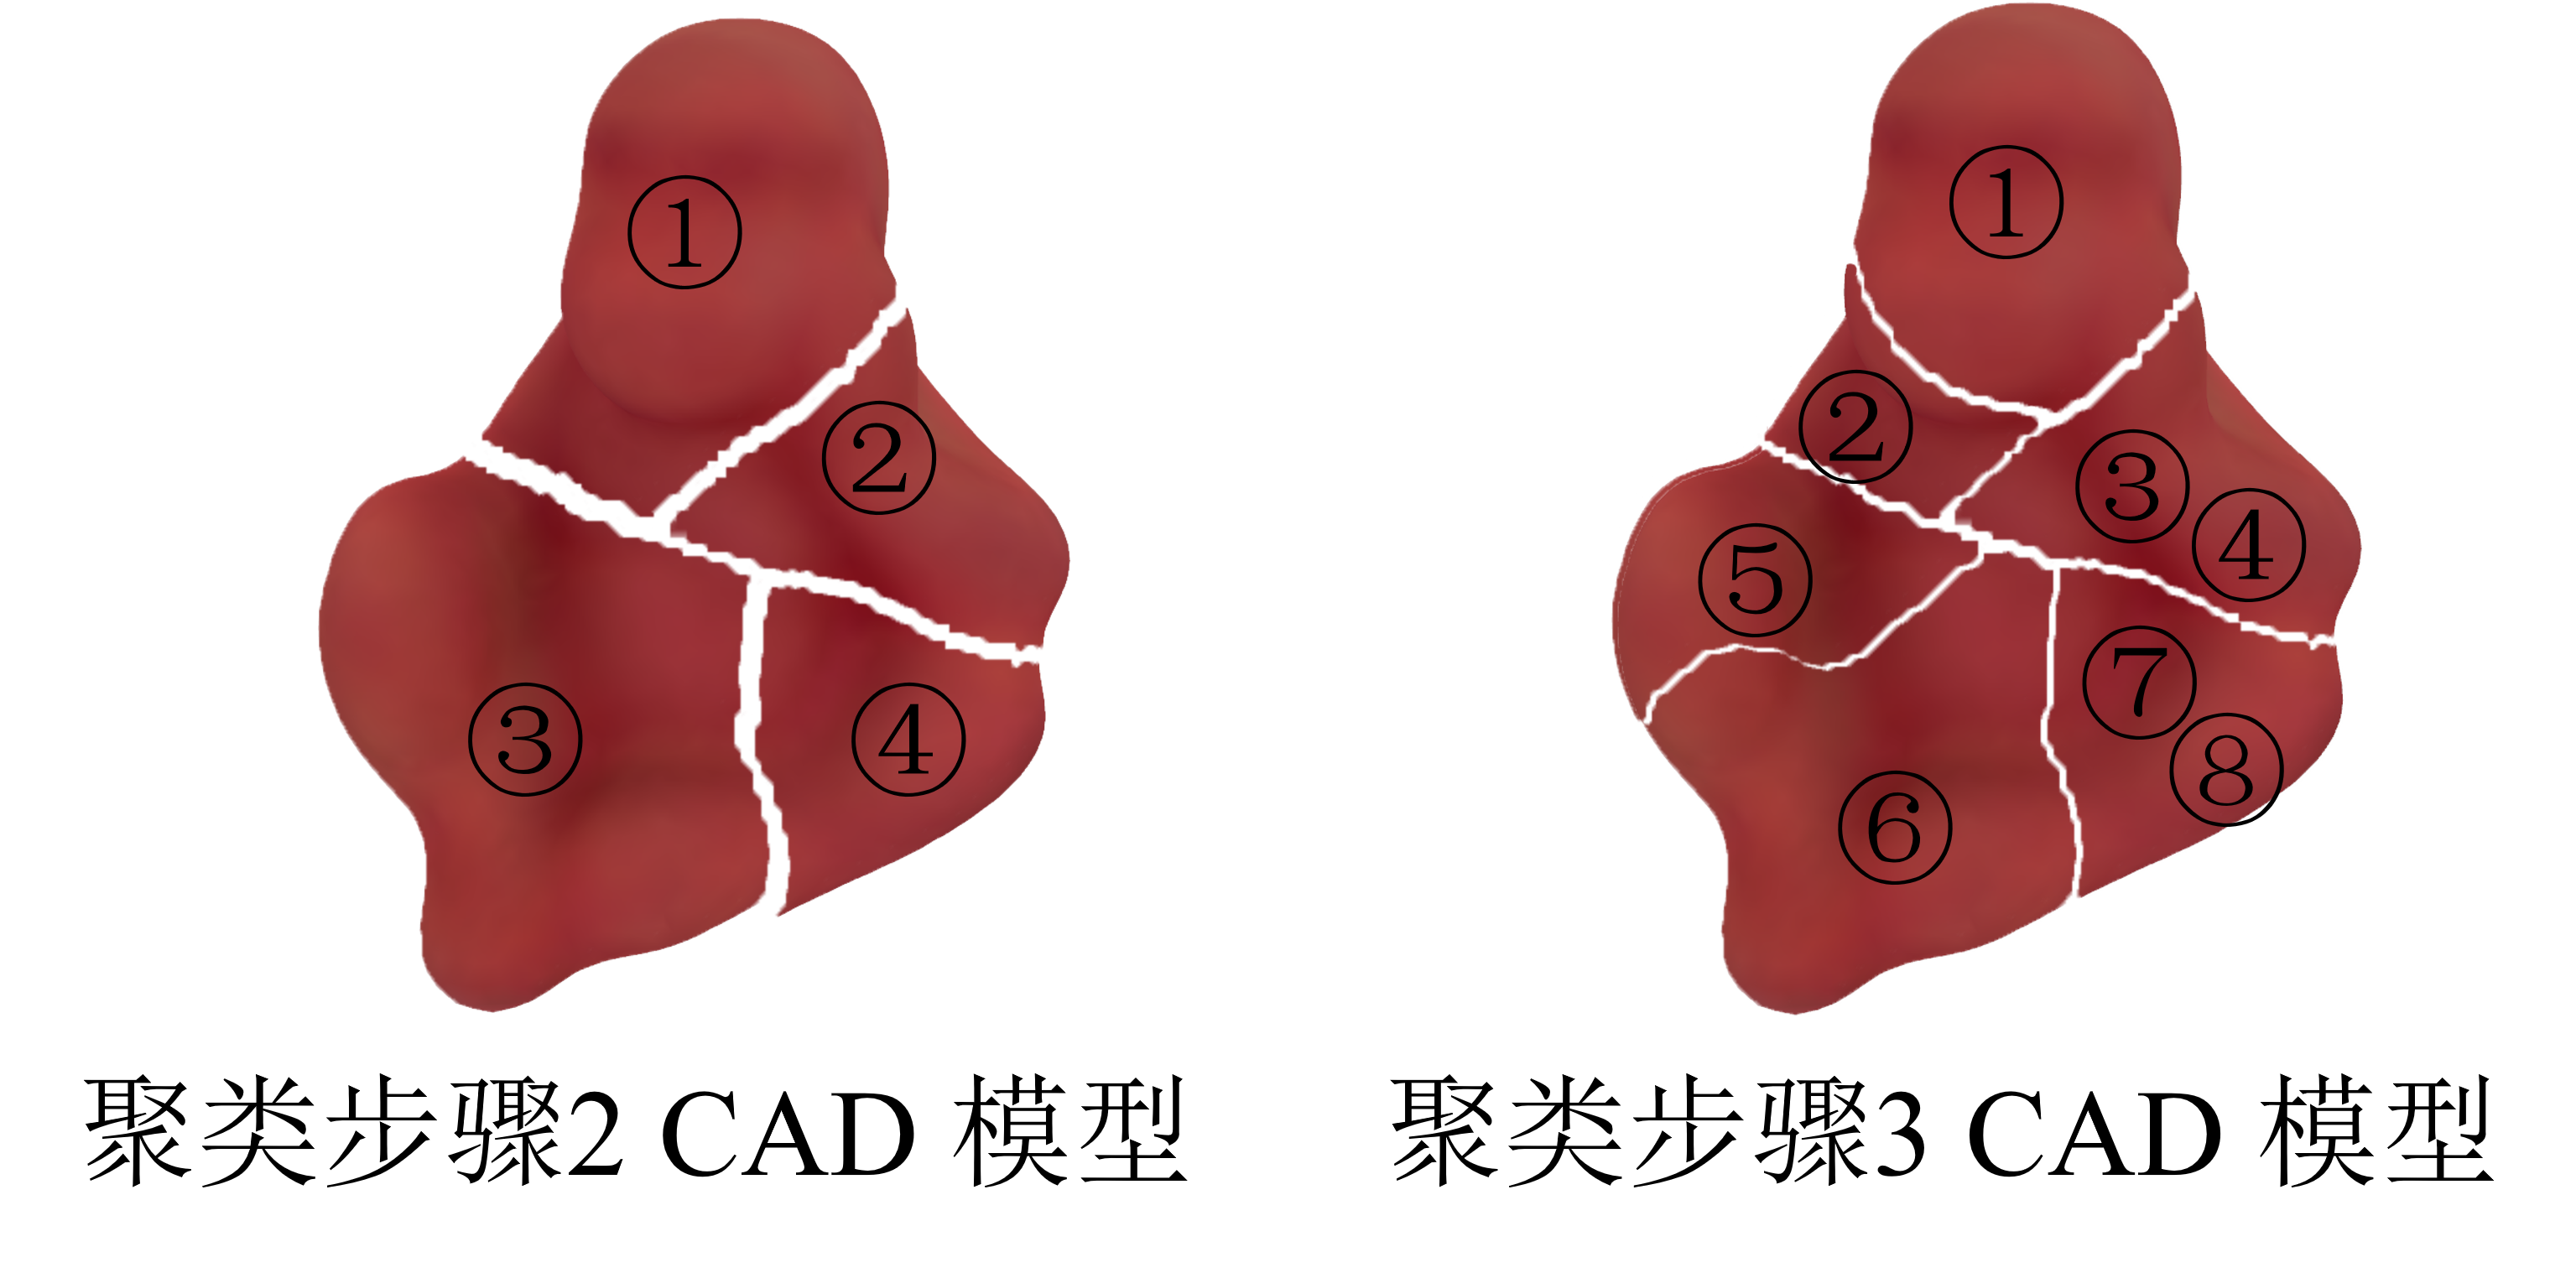
\includegraphics[width=0.5\linewidth]{hipose/聚类结果.png}
    \caption{聚类结果}
    \label{fig:聚类结果}
\end{figure}

我们将每次划分的两个子表面分别用0和1进行编码表示,将聚类步骤1到聚类步骤 $j$ 的编码组成一个二进制串作为该表面的划分编码。\autoref{fig:灰度图}展示了聚类过程中的编码,每一幅图中将二进制的$(0...0)_2$用黑色表示,$(1...1)_2$用白色表示。其他二进制数用相对应的灰度值进行可视化。下标表示二进制编码。

\begin{figure}[ht]
    \centering
    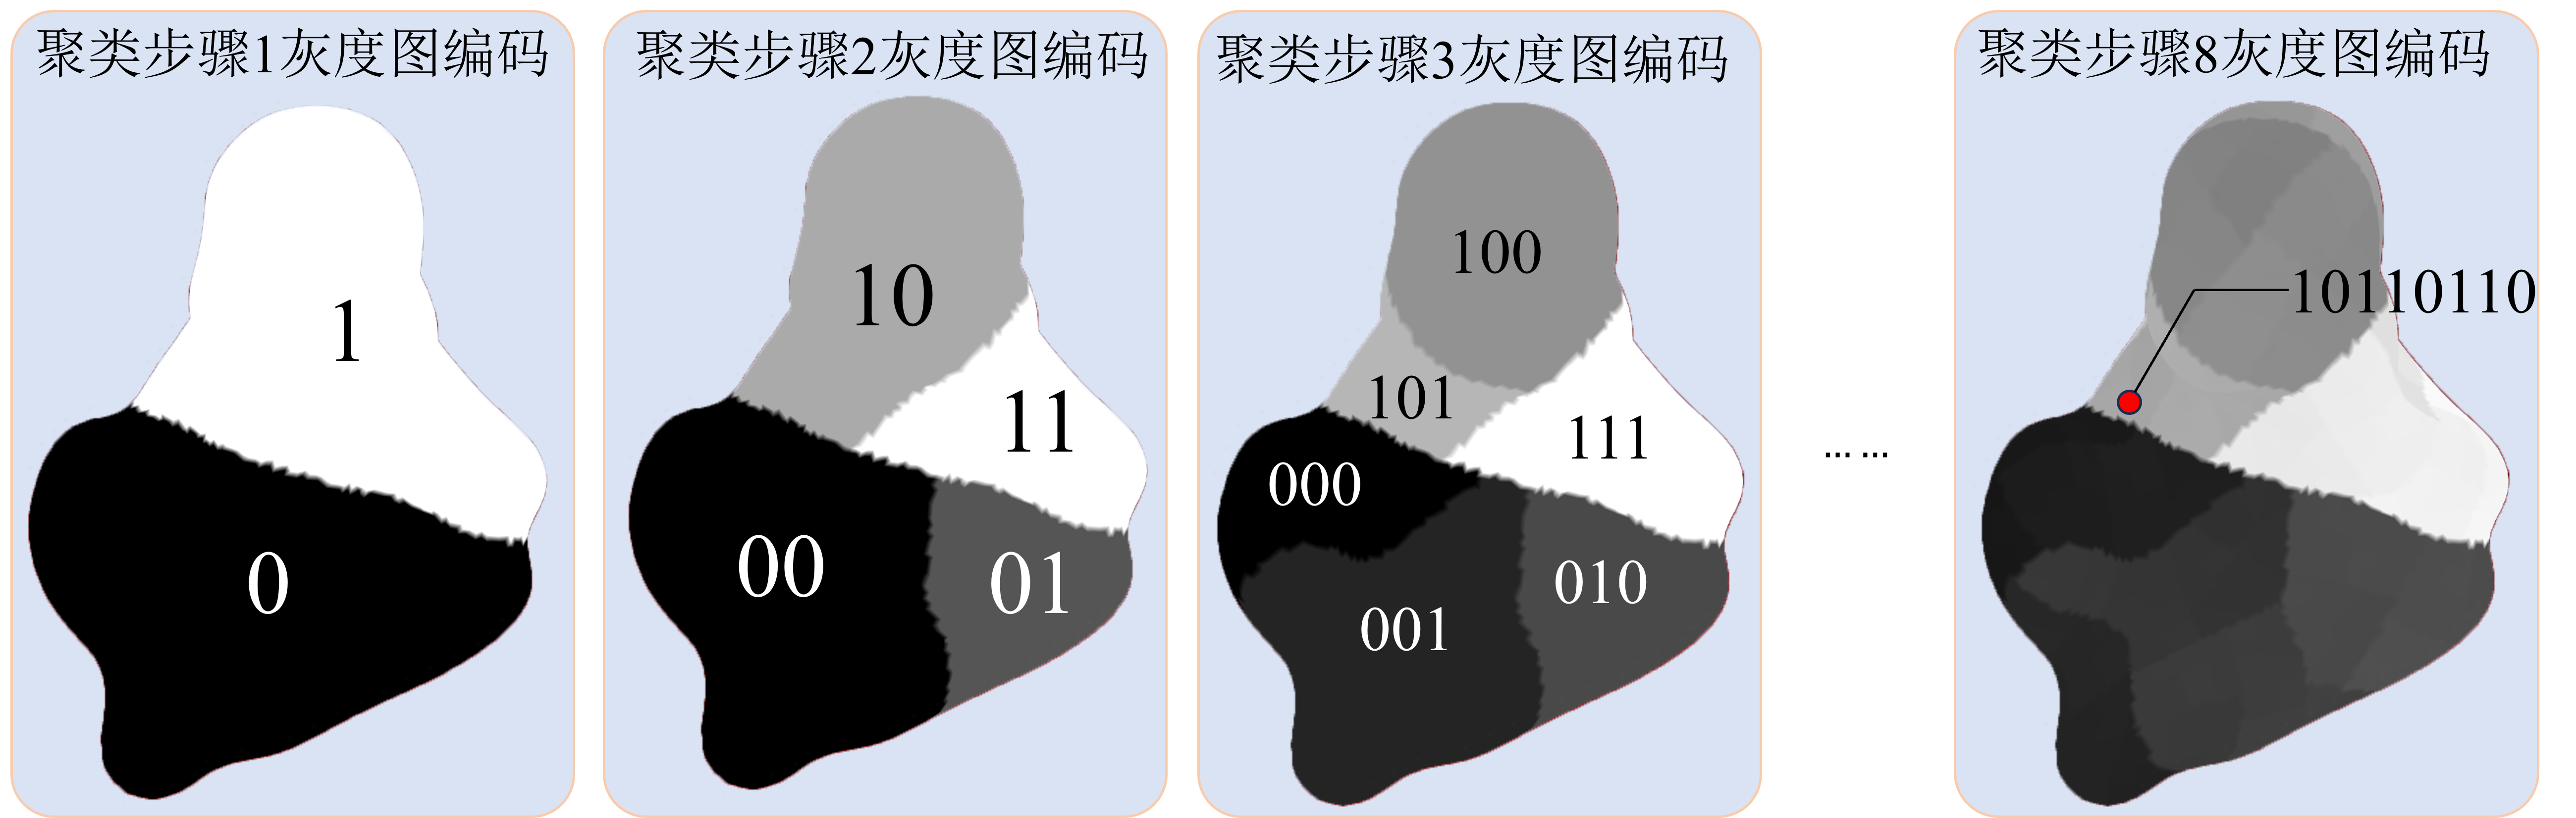
\includegraphics[width=1.0\linewidth]{hipose/灰度图.png}
    \caption{聚类过程的灰度图编码}
    \label{fig:灰度图}
\end{figure}

这个过程创建了一个分层编码,所有前 $n$ 比特相等的顶点,属于对象网格表面直到第 $n$ 次划分的相同子表面。换句话说,一个二进制编码 $\mathbf{c}$ 描述了一个从粗到细的物体表面的划分过程。当二进制编码位数足够多时,二进制编码所对应的物体表面面积足够小,则可认为二进制编码与物体表面坐标形成一一对应关系。

二进制编码的每一位都可以都可以用一个掩码(mask)进行表示,聚类步骤 $n$ 的结果可用 $n$ 个掩码进行表示。如\autoref{fig:坐标编码映射}所示,利用 $n$ 个掩码的相同位置的 01 值得到该图像像素点所对应的二进制编码,通过查表可得到对应的物体坐标系坐标。相反地,物体坐标系坐标也能够通过查表获取对应的二进制编码,进而构造出$n$个掩码作为训练标签。

\begin{figure}[ht]
    \centering
    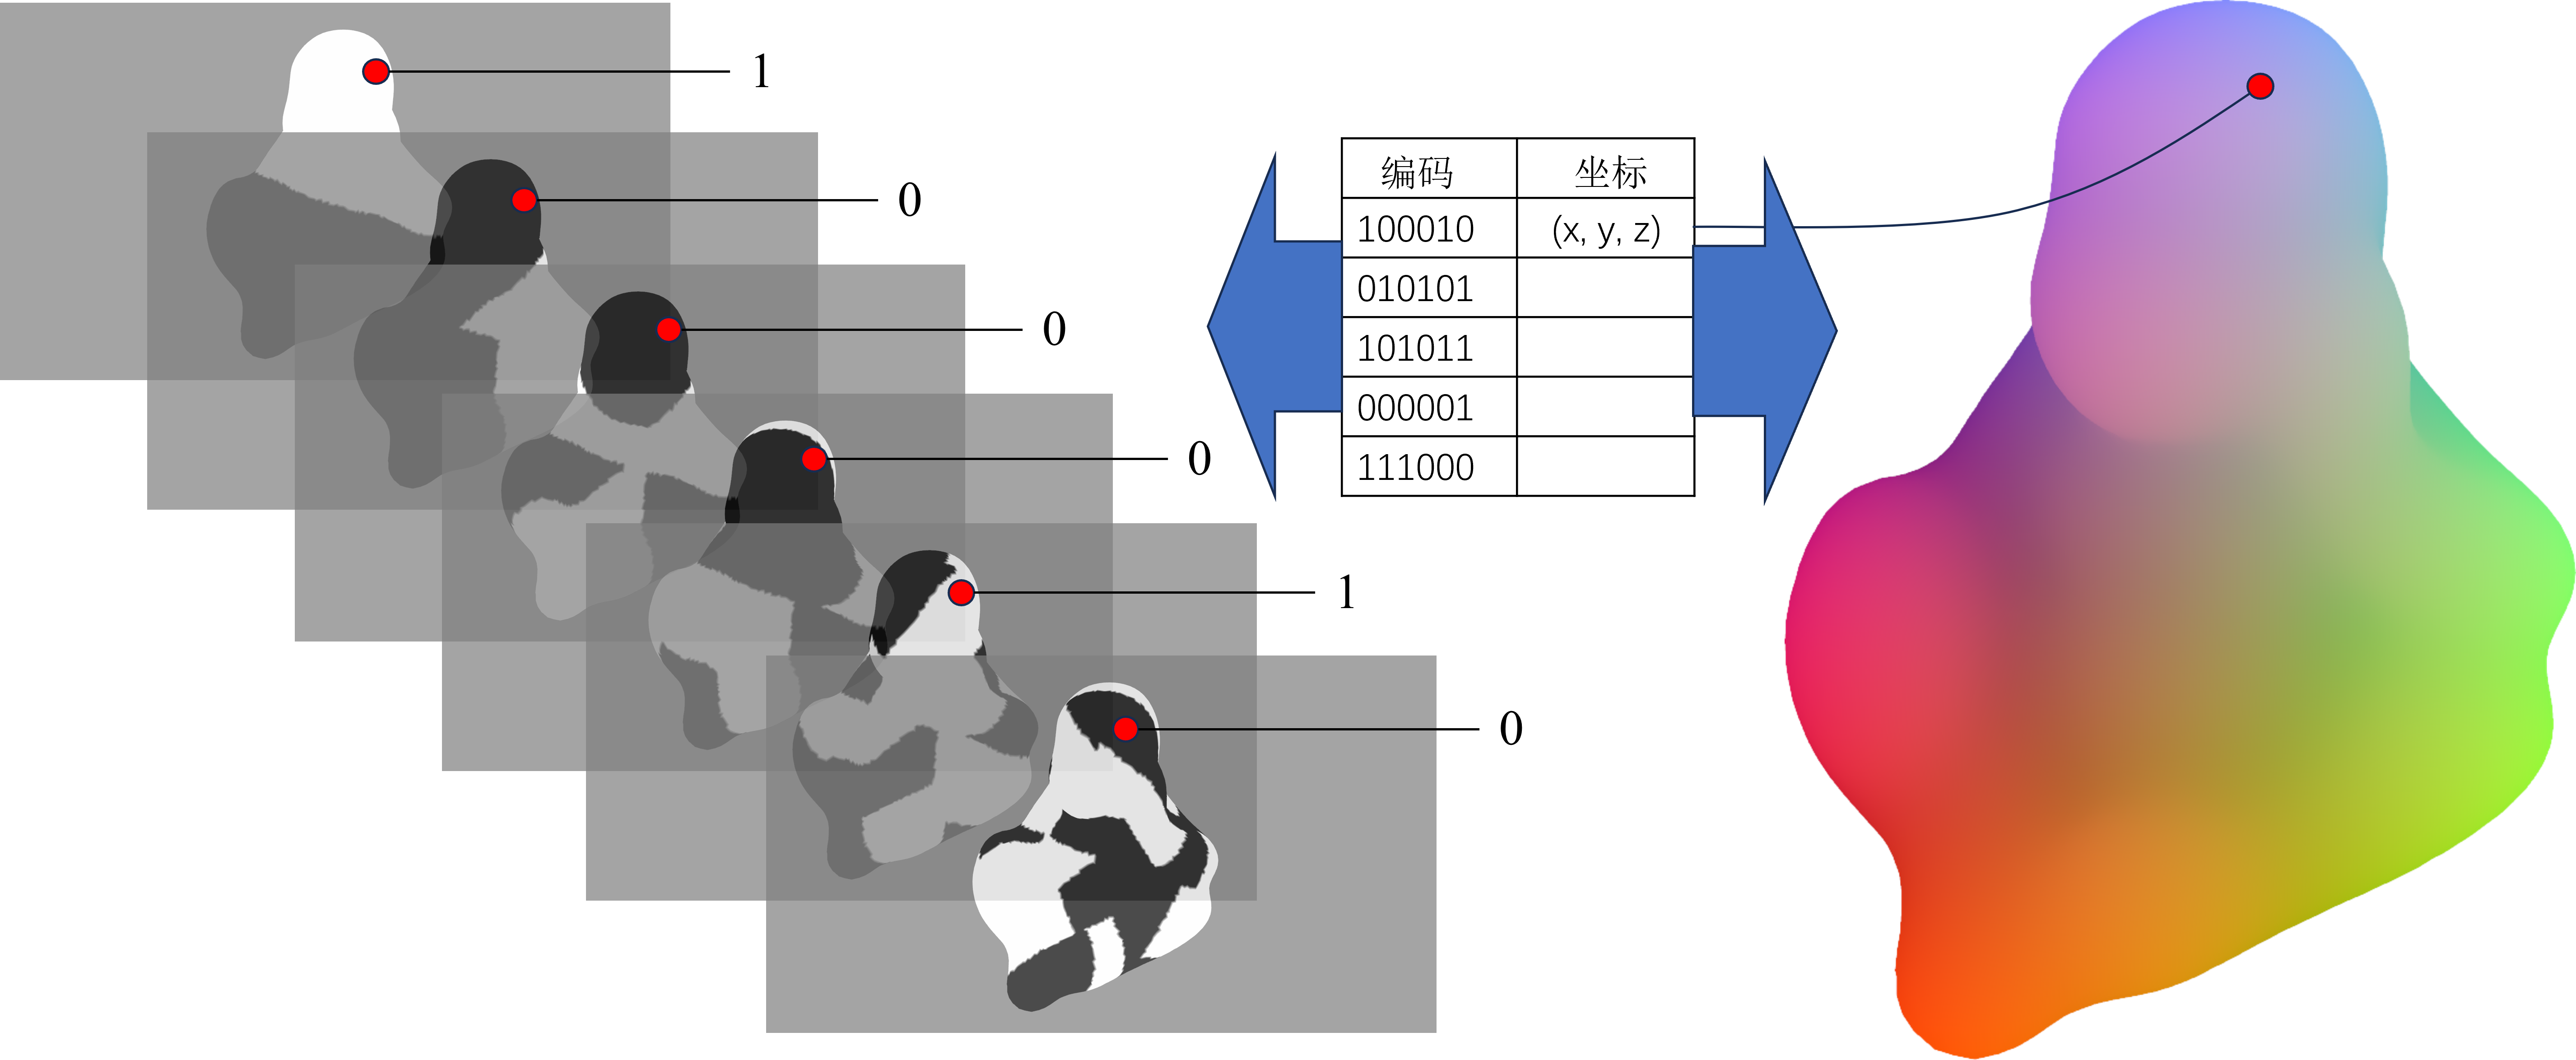
\includegraphics[width=0.75\linewidth]{hipose/坐标编码映射.png}
    \caption{坐标编码映射}
    \label{fig:坐标编码映射}
\end{figure}

\par 让网络学习二进制编码可以保证得到的物体坐标系坐标一定位于物体表面。此外,对于一个 $d$ 位的二进制编码,网络仅需要学习 $d$ 个二进制值,而直接使用物体坐标系坐标需要网络在$\mathbb{R}^3$上进行学习。

用物体坐标系坐标作为标签的方法用RGB图储存某张输入图片对应的物体坐标系坐标,二进制编码也能够使用RGB图进行存储。一般来说,对于单个物体,使用10位二进制编码已有足够高的精度,ZebraPose使用16位二进制编码。对于RGB图像的每个通道,都能够存储8位二进制编码,16位二进制编码能够只用红色和绿色两个通道就能够完成存储。如\autoref{fig:存储}所示,左侧为观测图像,右侧为转换为RGB格式的二进制编码存储图。

\begin{figure}[ht]
    \centering
    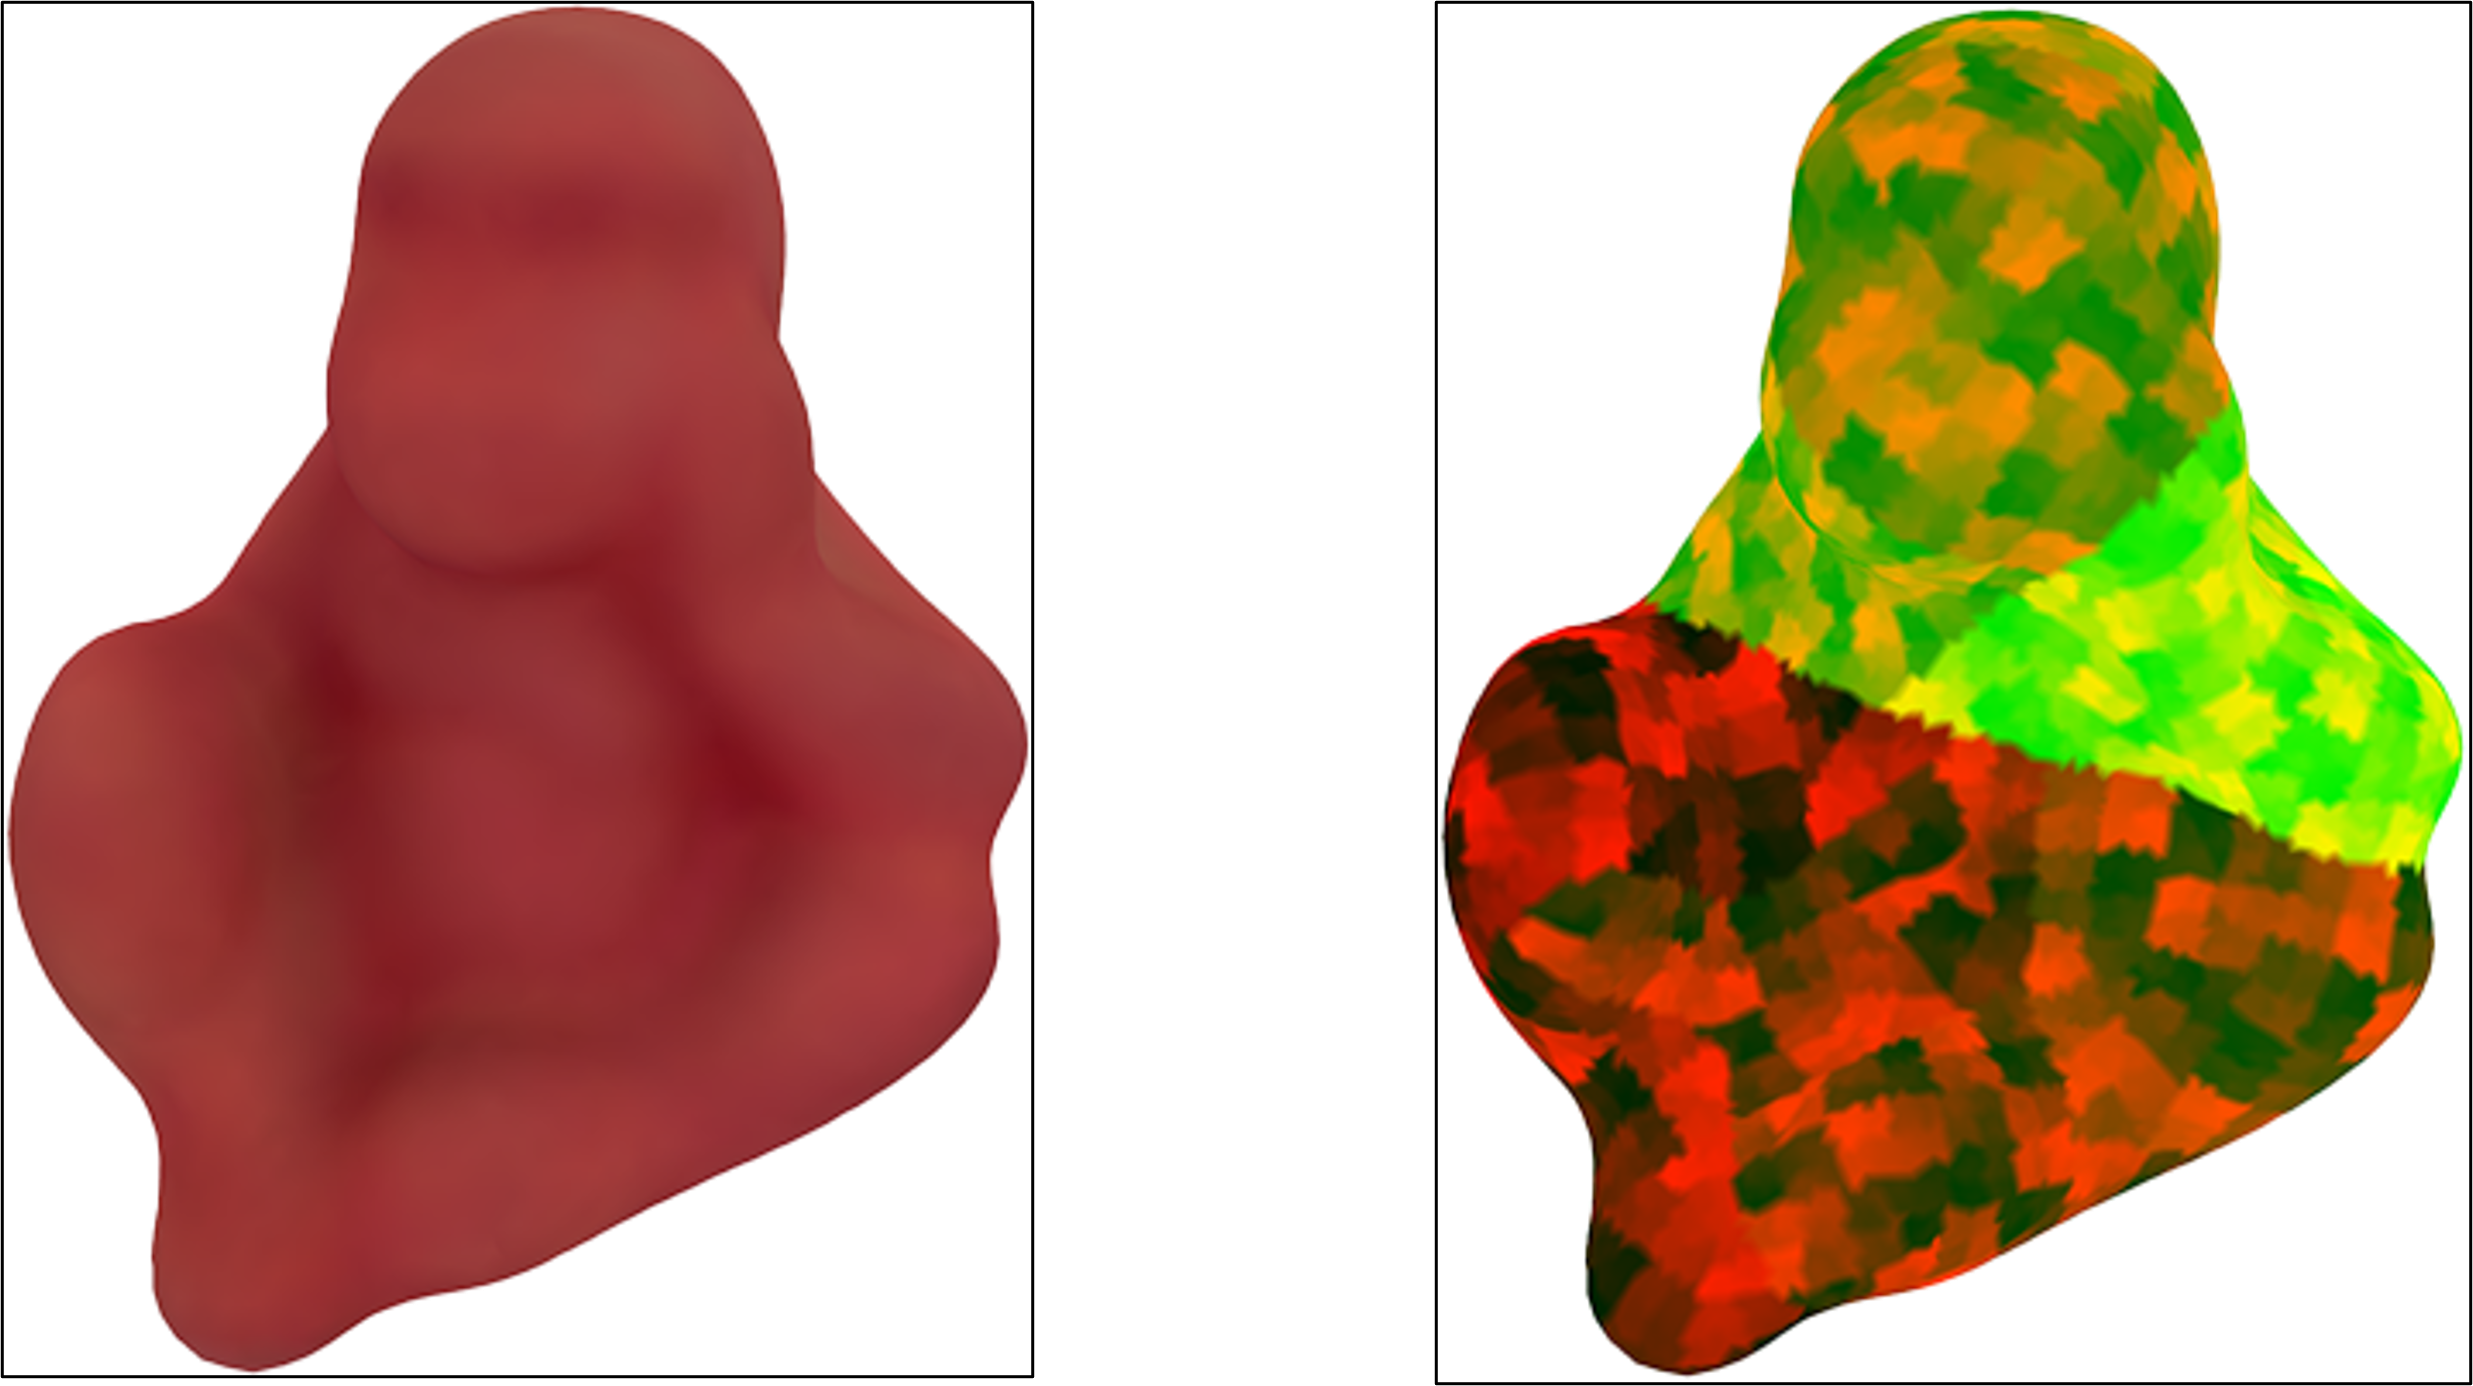
\includegraphics[width=0.5\linewidth]{hipose/二进制编码存储.png}
    \caption{图像与对应的转换为RGB格式的二进制编码存储图}
    \label{fig:存储}
\end{figure}